% Alles zur Hardware und unseren Modifikationen
% Zuständig: Mihael
\chapter{Hardware}
\label{sec:hardware}
\section{Elegoo Tumbller Kit}
\label{subsec:elegoo_tumbller}
Um den Hardwareaufbau so einfach wie möglich zu gestalten,
entschieden wir uns dafür,
fertig entwickelte Kits online zu bestellen und dann zu modifizieren.
%
Die Wahl des Kits fiel letztendlich auf den ``Tumbller'' von Elegoo (Siehe Abbildung \ref{fig:elegoo_tumbller}).
%
Der Tumbller ist ein zweirädriger Roboter, welcher auf einer Ache balanciert.
%
Zur Kontrolle des unmodifizierten Kits gibt es eine Smartphone-App,
welche die Roboter über Bluetooth fernsteuern kann.
%TODO genaue Hardwarebeschreibung des Kits
%
Da wir die Roboter über WLAN steuern wollten, 
und die Tumbller-Kits standardmäßig nur eine Bluetooth-Erweiterung eingebaut haben,
haben wir die mitgelieferten Arduino Nano durch ESP32-Boards im Arduino Nano-Format ersetzt.
% TODO Spannungsunterschiede Arduino Nano vs ESP
\begin{figure}[H]
    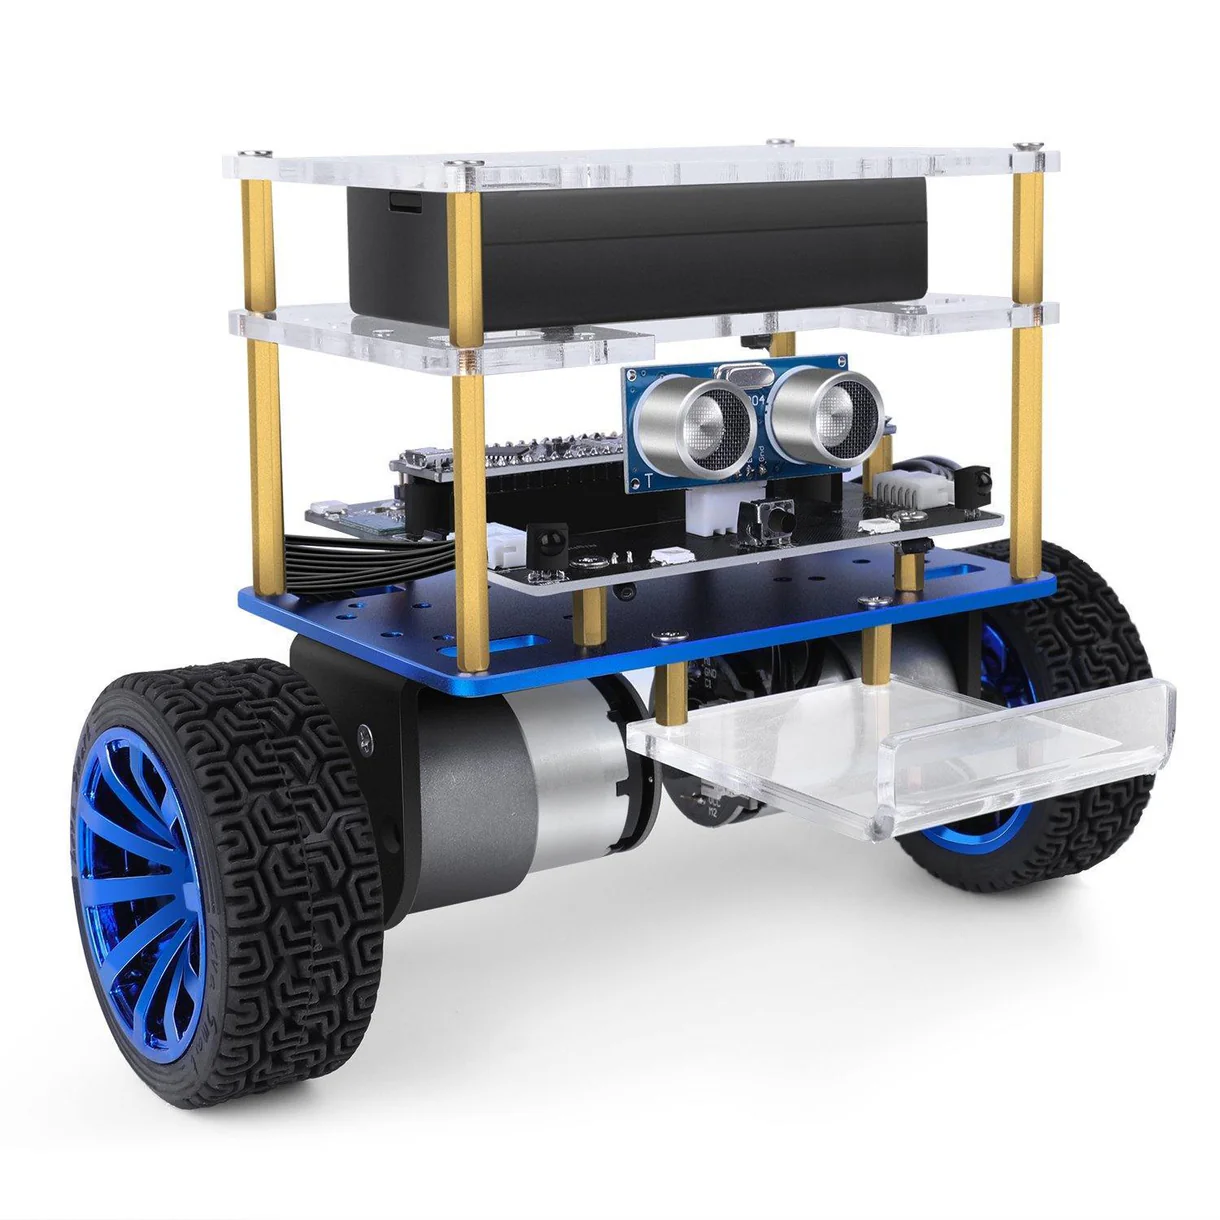
\includegraphics[width=0.7\textwidth, center]{img/elegoo_tumbller.png}
    \caption{Rendering des Elegoo Tumbller}
    \label{fig:elegoo_tumbller}
\end{figure}
\begin{sidewaysfigure}
    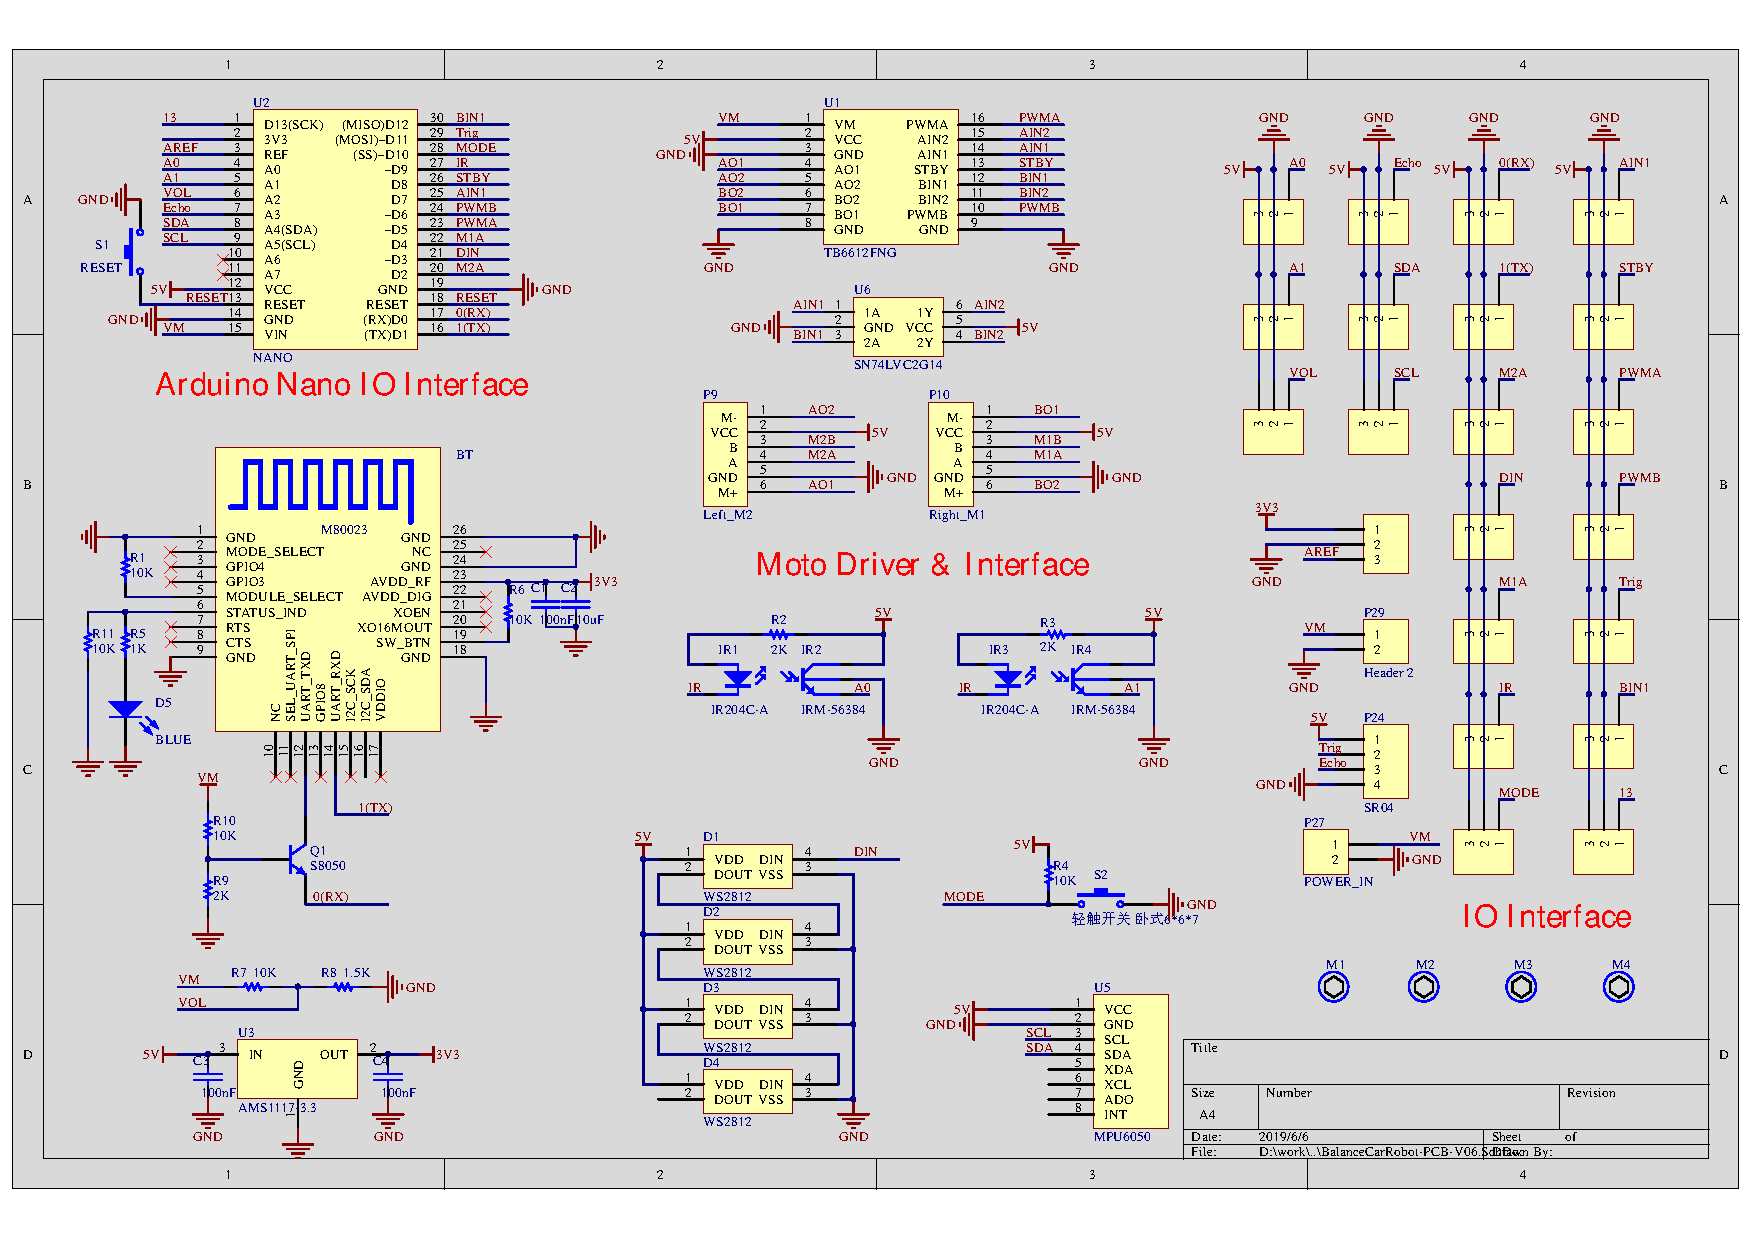
\includegraphics[width=\textwidth, center]{img/elegoo_tumbller_original_circuit.pdf}
    \caption{Originaler Schaltplan des Tumbllers (TODO: neu zeichnen)}
    \label{fig:elegoo_tumbller_original_circuit}
\end{sidewaysfigure}

\section{Arduino Nano zu ESP32 Nano}
\label{subsec:arduino_to_esp32}
Der Wechsel zum ESP32 Nano lief nicht reibungslos wie erhofft da,
obwohl der ESP von Arduino das "gleiche Gehäuse" verwendet 
es jedoch zu einigen Unterschieden in den Pins kommt. 

% TODO änder die pins aufs wichtige
\begin{figure}[H]
    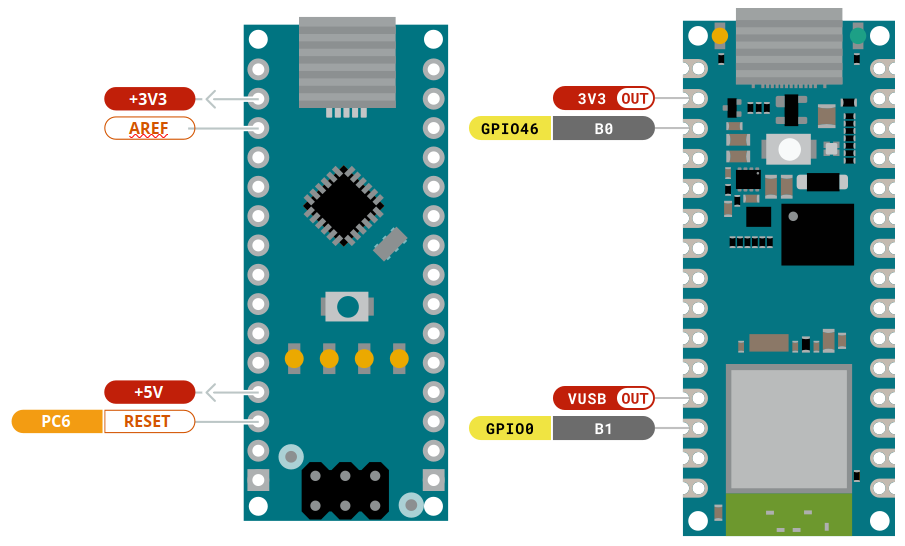
\includegraphics[width=\textwidth, center]{img/nano-differences-m.png}
    \caption{Hervorgehobene Pin out zwischen Arduino und ESP32 nano}
    \label{fig:nano_boards}
\end{figure}

Zwischen den Boards herrschen am relevantesten diese Unterschiede.
\begin{itemize}
    \centering
    \item Pin 3 von \texttt{AREF} zu \texttt{GPIO46} und \texttt{Boot0}.
    \item Pin 12 von \texttt{+5V} zu \texttt{VUSB} oder \texttt{VBUS}.
    \item Pin 13 von \texttt{RESET} zu \texttt{GPIO0} und \texttt{Boot1}.
\end{itemize}

Der Pin 3 von \texttt{AREF} ist unproblematisch aufgrund dessen dass,
es zu einem ungenutzten I/O Interface führt und somit keinem weiteren Besorgen.

Pin 12 ist muss etwas Achtung gegeben werden, weil der \texttt{VBUS} im Vergleich zu \texttt{+5V} als
direkte Führung von der Versorgung aus der USB Schnittstelle bedacht wurde und 
dadurch nicht weiter geregelt wird vom Board. Deswegen wird empfohlen den VBUS 
nicht mit anderen Pins am Nano kurz zuschließen, jedoch wenn der ESP32 über den VIN Pin versorgt ist, 
wird der Pin deaktiviert und sollte keine 5V von der USB Schnittstelle liefern können. 
Weiteres verhalten darüber hinaus ist dokumentiert.
Mehr dazu und der anderen Betriebsspannung ist in Abschnitt \ref{subsec:problem_betriebsspannungen} zu finden.

Pin 13 sollte keine Probleme machen da es zu einem offenen Schalter geht,
der ursprünglich den \texttt{RESET} Pin betätigt hätte und sonst offen liegt. 
Beim ESP32 würde der Schalter dafür sorgen das zum Boot Mode gewechselt werden kann, 
oder gewöhnliche Operationen mit \texttt{GPIO0}. 
Jedoch kam es zu Störungen an diesem Pin trotz internen Pull-up-Widerstand, 
wodurch wir den Pin entfernt haben mehr dazu siehe Abschnitt \ref{subsec:gestoert_boot}.

\section{Guide}
\label{subsec:hardware_guide}
Die Aufgabe von \textit{Guide} ist es,
mithilfe eines LiDAR-Sensors (Siehe Kapitel \ref{subsec:ueberblick_lidar}) die Umgebung nach Hindernissen
und den anderen Robotern abzusuchen.
%
Die vom LiDAR gesammelten Abstandsdaten werden über eine TCP/IP Websocket-Verbindung
an einen zentralen Server weitergegeben,
welcher diese weiter verarbeitet.
%
Um den LiDAR-Sensor zu montieren,
haben wir das Fahrgestell leicht modifiziert
und die oberste Ebene (mit dem Akku) erhöht,
um Platz für Schrauben zu schaffen.

\section{Tamerlan \& Bambi}
\label{subsec:hardware_tamerlan_bambi}